\documentclass[12pt]{article}
\title{Sophisticated Web Application Using Ajax Technology}
\author{Cl\'ement Beffa [clement.beffa@eplf.ch]}
\date{\today}

\usepackage{url}
\usepackage{graphicx}

\begin{document}

\maketitle

\section*{Overview}

The project should improve the current web interface on many aspect as design (one of the main factor which drives consumer choice), responsiveness (using asynchronous technique) and functionality (map integration for gps enabled sensor).  

\section*{Design and architecture}

\subsection*{Client side}

On of the core problem faced when using AJAX\cite{ajax} technology is the poor browser support and compatibility across different vendors. Even by focusing only on the biggest vendors (IE, Firefox \& Opera) which aggregate 99\% of the user base, there is still much compatibility issues. In order to avoid dealing will this issues and be forced to have tweaks for every browser, a good solution is to use a Javascript library which will be use as a middleware between our code and the browser. Such Javascript library will allow us to easily access the DOM, to make AJAX request or even have some fancy visual effects (fade out,...). However, this induces a new problem: Which Javascript library to choose?
There are plenty of Javascript libraries on the Internet. Almost all of them are opensource, so licensing isn�t an issue. This is a brief overview of the most famous :

\begin{itemize}
\item JQuery\cite{jquery}: A small understandable library which powerful functionality. Very active developer and gaining much popularity.
\item Prototype\cite{prototype}: Probably the most famous one due to RubyOnRails fame. Support everything we can expect but is a bit bloated. 
\item mootools\cite{mootools}: An ultra compact Javascript framework. Not so much user base.
\item Yahoo! User Interface (YUI)\cite{yui}: A proven library not so much use outside of Yahoo.
\end{itemize}

Considering those different libraries, JQuery was chosen as it has enough functionality for this project but remains quite small (15kb). Moreover, JQuery has a nice and powerful syntax which make code easy to write and read afterwards.

\subsection*{Server side}

AJAX techniques require data exchange between the client and server made by the Javascript on the client side. Although the X in AJAX means XML there is other way to exchange this data. On of the popular one, is to use JSON (JavaScript Object Notation) which send directly Javascript object. This is more efficient for the Javascript code on the client, however XML was preferred as it is more modular and allow to do at the same time a webAPI to access GSN sensors. We made something close to REST api entirely in XML so it would be more simple for us and people using the api to use it.

As early as the first week, the basic XML api was built in jsp in order to start the javascript interaction. It was used for a while then replaced by a servlet at location \emph{/gsn} to avoid using any jsp at all.

\section*{Implementation}

\subsection*{Javascript files}

For rapid development, we reused many piece of existing javascript code which are in the js folder. 

The following files are part of the webapp :

\begin{itemize}
\item jquery-latest.pack.js: The main jQuery library. We are using directly a version compiled from the svn as there were some fixes we needed which aren't in the latest version yet.
\item jquery-dom.js: An extension to jQuery which allow easy dom creation written like \$.DIV({"class":"test"},"content");
\item jquery.history.js: An extension to jQuery to manage the hash part of the location url (index.html\#hash). It is used to allow the page to be fully static html but still support the browser back button and bookmarking of specific part of the page.
\item dimensions.js: An extension to jQuery to know the page width and height. Used only in fullmap.html in order to have the container with vsboxes at the right size.
\item  datepicker.js: Customized extension of jquery used for the datetime helper
\item  jquery-tooltip.js: A plugin to have better tooltip than the browser default behaviour which is used for descriptions
\item  gsn.js: Our core javascript code. Explanation in the next subsection.
\end{itemize}

\subsection*{gsn.js core function}

Almost all of gsn JavaScript code is regrouped inside gsn.js. It written using a JavaScript Object Notation and use a GSN object to reduce conflict with any future addition of JavaScript code. \emph{vsName} which is the name of the virtual sensor (text) is considered as unique, which explain why it is so much used as parameter. Most of the ajax call goes to the \emph{/gsn} servlet. The data part use the \emph{/data} servlet for retreiving data. Binary and image are accessed through the \emph{/field} servlet and webinput upload goes to the \emph{/upload} servlet.

Here is a brief explanation of the core variables and functions:

\begin{itemize}
\item GSN.context: Define on which page of gsn we are (home, data, map or fullmap)
\item GSN.load(): Initialize a page load (begin, tab click \& back button)
\item GSN.msgcallback(): Callback method when the webupload iframe finish
\item GSN.nav(page): Click on the top navigation bar
\item GSN.menu(vsName): Click on the virtual sensor on the left bar
\item GSN.loaded: Is true after the first load of XML info which call GSN.init()
\item GSN.init(): Initialize the gsn title and leftside menu
\item GSN.updatenb: A counter to prevent multiple instance of GSN.updateall().
\item GSN.updateall(): Ajax call to update all the sensor display on the page and the map
\item GSN.addandupdate(vsName): Add a vsbox if it doesn't exist, bring it to front and update it
\end{itemize}

The virtual sensor information (dynamic, static and structure) are regrouped in a div box called the vsbox. This div have the class .vsbox and .vsbox-{the virtual sensor name}. They will be put in the container specified by GSN.vsbox.container. Here are the function of the GSN.vsbox.* part:

\begin{itemize}
\item GSN.vsbox.container: The container to put the vsbox (default "\#vs")
\item GSN.vsbox.add(vsName): Create an empty vsbox
\item GSN.vsbox.bringToFront(vsName): Bring a vsbox at the beginning of the container
\item GSN.vsbox.update(vs): Update and show all the data of the vsbox
\item GSN.vsbox.remove(vsName): Remove the vsbox from the container
\item GSN.vsbox.toggle(...): To manage the click on tab
\end{itemize}

All the functionality used to display the virtual sensor on the google map are regrouped in the GSN.map.* part. Here is the core functionality:

\begin{itemize}
\item GSN.map.loaded: Is true after the initialisation of the google map.
\item GSN.map.markers : Array containing the displayed markers
\item GSN.map.highlighted : Is the index of the focused marker or null.
\item GSN.map.highlightedmarker : Is the green marker
\item GSN.map.init(): Initialize the google map
\item GSN.map.userchange(): Callback after any map change (zoom and map move) and vs toggle to update \#hash of URL
\item GSN.map.zoomend(..): Callback after any zoom change, Used for the tricked followed marker
\item GSN.map.trickhighlighted(): Followed marker and top of the others
\item GSN.map.autozoomandcenter(): Auto-zoom and center on the visible sensors
\item GSN.map.addMarker(vsName,lat,lon): Add a vs marker on the map
markerIsVisible(vsName): Return if a marker is visible
toggleAllMarkers(): Toggle all marker (visible or not)
toggleMarker(vsName): Toggle marker (visible or not)
\item GSN.map.updateMarker(vsName,lat,lon): Update a vs marker position on the map
\item GSN.map.followMarker(vsName): Highlight a marker, Stop it if called with null name
\item GSN.map.showAllMarkers(): Zoom out to see all markers
\end{itemize}

The functionality in the data webpage are regrouped in the GSN.data.* part and where only bugfixed and slightly improved so they won't be covered in this report. The remaining GSN.util.* functions are basic formatting piece of code that don't need any explanations at all.

\subsection*{Problems faced}

\subsubsection*{Dropping tables}

The first version of the gsn webapp "template" was using tables for layout which is considered as bad by almost any webdesigner. Therefore, It was transformed to a layout using only divs and css for styling. The advantages is cleaner html code, thus easier to understand, more flexibility, as changing only the css could change the whole look \& feel, and faster as the size is smaller and the css file could be cached by the client browser. It was quickly rewritten from scratch to match the current gsn website style.

\subsubsection*{IE showstopper}

After the first week of implementation, we had a big problem. Some of the functionality used in jQuery library weren't compatible with IE. They were some rare XML parsing which broke totally. Hopefully, with the help of the jQuery team, it was resolved. Therefore, we switched from jQuery 1.0 to the jQuery from the svn as it was the only fixed version.

Another IE only bug caused problem, because Ajax request in IE are locally cached like any normal http request. Therefore, the webapp wasn't refreshing even if the javascript was working fine and making ajax calls. It was easily resolved by adding to the XML api servlet various http header (Expires, Cache-Control,..) to avoid any caching at all.

\subsubsection*{Retrieving dynamic data with ajax}

As the webapp is only static html files, the dynamic data has to be pulled from the servlet through JavaScript. It is done easily using the \emph{.ajax} function of jQuery. In the main \emph{GSN.updateall} function which update all virtual sensors data at every refresh, the webapp calls using ajax the servlet at \url{http://localhost:22001/gsn} using the following code:

\begin{verbatim}
$.ajax({ type: "GET", url: "/gsn", success: function(data){
	// use the �data� variable which contain virtual sensors data 
}
\end{verbatim}

As shown above, using ajax in jQuery is very straight forward. The retrieved data is in xml and formatted as below:

\begin{verbatim}
<gsn name="gsn" author="cb" email="cb@epfl.ch" description="none">
  <virtual-sensor name="vs" last-modified="1171105166765">
    <field name="temp" type="long" description="none">-5</field>
  </virtual-sensor>
</gsn>
\end{verbatim}

After retrieving the xml data, it is parsed with the \emph{\$()} function of jQuery which support xml data similarly to inline html. The syntax looks as below with the data variable being the ajax reply from the servlet:

\begin{verbatim}
$("virtual-sensor",data).each(function(){
  var vsname = $(this).attr("name");
});
\end{verbatim}

When the \emph{GSN.updateall} function finished to parse xml and update the inline html with the new virtual sensors data, the standard Javascript function \emph{setTimeout()} is used in order to call the \emph{GSN.updateall} function again for the next refresh.  

In addition, when clicking on the right side menu on a virtual sensor, an ajax call is made as well. The data of the clicked virtual sensor is retrieved using \url{http://localhost:22001/gsn?name=vsname}. The logic is the same than during a \emph{GSN.updateall} but only the specified virtual sensor is in the xml data. Using the same JavaScript code, it will update only the specified virtual sensor box.

Not much can go wrong with those ajax calls. As we specified the reply format, the reply will always be fully understood by the JavaScript parsing. The worst that might happen would be that the servlet died. In that case, the ajax query will timeout and never success which will stop any further update and the ajax indicator (animated gif) will turn forever which shows that something went wrong during xml data fetching. In no case, the client browser will freeze or crash. The user could actually still use the gsn webapp, but will not see any new update to the data.

\subsubsection*{XML formatting of virtual sensor}

As explained in the design choice, the gsn webapp use an xml api to give data. All virtual sensor informations are regrouped into a single \emph{virtual-sensor} block. All the different types of data (dynamic, structure, predicate,..) is merged into a single entity as it is much more efficient than having to query multiple times the servlet. The overall size of a single block, as it is only text, costs far less than the latency of multiple queries. Moreover, the main gsn webapp page requires all types of data at the initialization, thus merging them make sense. 

Every type of data are mapped into the \emph{field} block following the rules below. Field names are converted into lowercase and fields are sorted by type in the same order than below.

To begin with, the \emph{virtual-sensor} block is opened with the following included attributes:
\begin{itemize}
\item name: Virtual sensor name (unique)
\item last-modified: Last-modified datetime in unix format
\item description: Virtual sensor description
\end{itemize}
Here is a sample of the xml output from the servlet:
\begin{verbatim}
<virtual-sensor name="vsensor1" last-modified="1171104402145" 
description="Virtual sensor">
\end{verbatim}

Then, the dynamic fields with their data are mapped from the output-structure block from the xml config of the virtual sensor into a unique field block. Below is a xml config sample:
\begin{verbatim}
<output-structure>
  <field name=" temperature" type="double"> temp somewhere </field>
</output-structure>
\end{verbatim}
It would be mapped into the following line in the xml output from the servlet:
\begin{verbatim}
<field name="temperature" type="double" description="temp 
somewhere">-5.1</field>
\end{verbatim}

An additional dynamic field is added with the timestamp in unix format which is like the following xml sample:
\begin{verbatim}
<field name="timed" type="long" description="The timestamp associated 
with the stream element">1171451930547</field>
\end{verbatim}

Afterward, the static predicate fields are mapped from the adressing block from the xml config of the virtual sensor into a unique field block as well if they exist. Below is a predicate xml config sample:
\begin{verbatim}
<addressing>
  <predicate key="LATITUDE">37.4</predicate>
</addressing>
\end{verbatim}
It would be mapped into the following line in the xml output from the servlet:
\begin{verbatim}
<field name="latitude" category="predicate">37.4</field>
\end{verbatim}

Additionally, the webinputs block from the xml config of the virtual sensor are mapped into a unique field block if they exist. They are not kept hierarchically by command anymore. Below is a xml config sample:
\begin{verbatim}
<web-input password="test">
  <command name="cmd1">
    <field name="control" type="*binary:2mb">Binary upload</field>
  </command>
</web-input>
\end{verbatim}
It would be mapped into the following line in the xml output from the servlet:
\begin{verbatim}
<field command="cmd1" name="control" category="input" 
type="*binary:2mb" description="Binary upload"/>
\end{verbatim}

Finally, the \emph{virtual-sensor} block is closed.
\begin{verbatim}
</virtual-sensor>
\end{verbatim}

Mapping all these different types into the same field block syntax is easier to parse by jQuery and allow reuse of code for similar functionality, like between dynamic and static fields.

\subsubsection*{Highlighted marker on Google map}

The code around GSN.map.trickhighlighted() can look quite suspicious. Why so much code and diverse variables just to highlight a marker on Google map? Changing from one type of marker to another doesn't require all this. It could have been made easier, but then when you zoom out you might not see the highlighted marker if it's surrounded by many other markers. It is due because Google map doesn't allow to specify the z-index of a marker and automatically order them by their latitude. Thus the marker with the lowest latitude will be shown on top of the others one. 

This behaviour can be changed by using a trick which is to use a marker with an offsetted latitude and an offsetted marker image which will always be at a lower latitude than the other markers. Thus always be on top of them. It is offsetted depending of the zoom level and the normal marker height. With this trick, the highlighted marker is popping out of crowd as shown on the left side image. 
\begin{center} 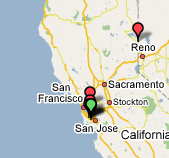
\includegraphics{gsn2_hightrick1.png} 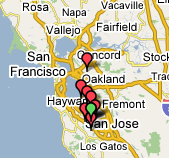
\includegraphics{gsn2_hightrick2.png} \end{center}
The only drawback of this technique is that it might look weird sometime because of the shape of the marker. As the right side image shows, the spike of the highlighted market is on top of the one bellow. Anyway it isn't that frequent and the benefits when zoomed out in a dense area of marker are worth it.

\subsubsection*{Bookmarking and back button support for Ajax website}

When webapp use ajax technique, one of the key feature of the browsing experience is broken: the URL. With ajax calls made without a page load, the state of the current webpage isn't related to the URL anymore. It breaks the back button feature of any browser, moreover that the current webpage can't be bookmarked properly. As those feature are essential to a website, it is needed to found a way to mimic them. The solution is to use the hash part of the URL : \url{http://server.com/index.html#hash}. The hash part is easily modified through javascript without a page load and is considered as a page change by every browser which means the back button feature works. In addition, an url with a hash part can be bookmarked and, with some javascript initialization, can restore the webpage in the same state than bookmarked. It was implemented using a jQuery extension as some tricky javascript code is required to make this functionality compatible with Internet Explorer. 

For example, URL in the gsn webapp when browsing the map part might look like the following:\\
\url{http://localhost:22001/#map,lt=38.17343267903539,lo=-121.9537353515625,z=8,vs=gpsvs:gps2:memorymonitorvs}

Such URL is fully bookmarkable and will initialize the webapp at the same state which allow people to share URL in order to show specific sensors. It is decomposed into several parameters which represent:
\begin{itemize}
\item \url{map}: which context/part of the webapp (could be home, data or map)
\item \url{lt=38.17343267903539}: latitude of the map when not in automatic mode
\item \url{lo=-121.9537353515625}: longitude of the map when not in automatic mode
\item \url{z=8}: zoom level of the map when not in automatic mode
\item \url{vs=gpsvs:gps2:memorymonitorvs}: shown virtual sensors when some are hidden
\end{itemize}

Nevertheless, the URL can become quite long with all these parameters include in it. However, it is not a problem as Internet Explorer support URL length up to 2048 characters. The alternative web browsers (FireFox, Opera \& Safari) are even better and support up to 100000 characters. 

\subsubsection*{Improved UI}

The general user interface was given much thought. The UI of the data part was highly customized. To simplify and to be more error prone, the datetime field was given some special helper shown bellow. 

\begin{center} 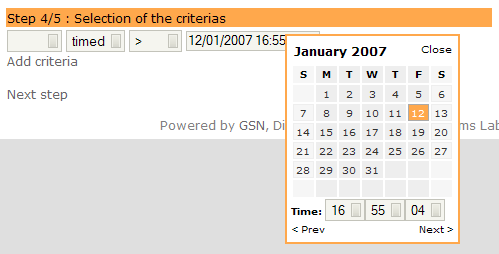
\includegraphics[width=0.6\textwidth]{gsn2_datetime.png} \end{center}

It allow the user to specify a date and time only with mouse click. It was proven to be much more quick that way. 

A waiting indicator was added during ajax calls when gsn refresh sensors fields or when data are retrieved in the data part. Such indicator are necessary in ajax application, otherwise the user will think nothing is happening, will get frustrated and might click multiple time which won't improve respond time.

\subsubsection*{Webinput upload to virtual sensor}

The ability to upload input to a virtual sensor, as shown below, was one of the last addition to the gsn webapp. 

\begin{center} 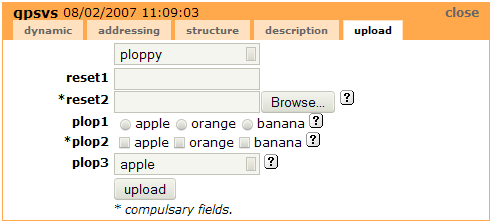
\includegraphics[width=0.6\textwidth]{gsn2_upload.png} \end{center}

For simplicity and modularity, the upload inputs are regrouped into subgroup which can be selected with the upper select box. Upload inputs are optional and specified in the sensor xml configuration, thus the tab only appear when it is specified. The different types are specified but are not enforced on the client side as it could be easily bypassed. 
The validation is done on the server side as client input should never be trusted. The following types have special input fields :

\begin{itemize}
\item \emph{binary}: file upload
\item \emph{radio}: radio button with limited choice
\item \emph{checkbox}: checkbox with limited choice
\item \emph{select}: drop down box with limited choice
\end{itemize}

The radio, checkbox and select types use the syntax like "radio:ele1|ele2" to specify the multiple choice. The binary field is limited by a maximum size specified in the type part with a syntax like "binary:Xmb". When the type begin with a star, it makes it compulsary. Here is a sample xml config which shown all the capabilities:
\begin{verbatim}
<web-input password="test">
  <command name="cmd1">
    <field name="reset1" type="byte" />
    <field name="reset2" type="*binary:2mb">Description</field>
    <field name="test1" type="radio:apple|orange|banana">one</field>
    <field name="test2" type="*checkbox:apple|orange|banana">two</field>
    <field name="test3" type="select:apple|orange|banana">three</field>          
  </command>
</web-input>
\end{verbatim}

An ajax like behaviour was require to give feedback to the user after the webinput upload. However, the XMLHTTPrequest object used to send ajax calls doesn't support file upload for security reasons. To bypass this limitation, a normal FORM element is used but use a hidden inline frame as a target. When the user clicks the submit button, the upload starts in the hidden IFrame to the destination \emph{/upload}. When the upload ends or breaks, the servlet reply back html code like the following code line. This javascript code calls back the parent window GSN core object which allow the webapp to give feedback to the user.

\begin{verbatim}
<script>window.parent.GSN.msgcallback('msg',code);</script>
\end{verbatim}

On the servlet side, the jakarta fileupload library was used to speed up developpement. A servlet translates the POST upload into XML-RPC format before sending it to the gsn system. The xml produced is similar to the following block lines. Normal fields are given in text format and binary fields are encoded in Base 64. 

\begin{verbatim}
<input>
  <vsname>gpsvs</vsname>
  <command>test</command>
  <fields>
    <field>
      <name>reset1</name>
      <value>test comment</value>
    </field>
    <field>
      <name>reset2</name>
      <value>ABQOBJREFUevQ18FNW9/3+C/q7tza+tXB ... AARK5CYII=</value>
    </field>
    <field>
      <name>test1</name>
      <value>banana</value>
    </field>
    <field>
      <name>test2</name>
      <value>orange</value>
    </field>
    <field>
      <name>test2</name>
      <value>apple</value>
    </field>
    <field>
      <name>test3</name>
      <value>orange</value>
    </field>
  </fields>
</input>
\end{verbatim}

The servlet takes care of keeping only the input fields of the activated, by the drop down menu, command. The xml ouput can be read in the \emph{sb.toString()} variable and as to be validated by the gsn system. The feedback is send to the user as explained before and correspond, in the servlet, to the \emph{msg} and \emph{code} variables. The \emph{msg} could be any text string but should escape single quote and will be displayed at the top of the webinterface. A \emph{code} higher than 200 is considered as an error and is shown in red to the user, otherwise it is in black. Nevertheless the code is not shown to the user in the current interface.


\subsubsection*{Porting from jQuery 1.0 to 1.1}

Porting the javascript from 1.0 to 1.1 wasn't straight forward. Some API function from jquery were removed to decrease complexity like \emph{\$().title} replaced by the generic \emph{\$().attr("title")}. The \emph{ \$(element,context) } wasn't working properly. I'm not aware if it's a new bug or or a feature yet. Anyway, the problem where solved using a different function: \emph{\$(context).find(element)}. 

Using the last version of jQuery is important for the speed improvement involved and simplify further update. Upcoming version won't have much more API change hopefully.

\subsection*{Testing \& Debugging}

GSN webapp was fully tested using the main browsers on the web: Internet Explorer, Firefox \& Opera. There wasn't any formal testing routine or unit testing. However, the core functionality were tested in the three browsers to ensure that they were working similarly.

After a month of implementation, the interface was quite advance however never tested with many sensors. When we added 40+ sensors, it became ridiculously slow. More than 15 seconds to show them. Javascript is slow and using some nice syntax feature of jQuery can be very expensive, especially the \$("") function! By refactoring the code, avoiding to use the more expensive function and much testing, the execution time was reduced to less than 2 seconds. A factor 10 improvement! However, as the number of virtual sensor could be even much more, it was decided to show only the ten first sensors on the front page which reduce the time even more. Later the speed was improved as well by updating jQuery to the new 1.1 version.

\subsubsection*{Javascript debugging}
With ajax webapp, the amount of complex javascript code is significant, thus it needs to be debugged and analyzed. Hopefully, a relatively new extension for FireFox called FireBug\cite{firebug} helps a lot.

\begin{center} 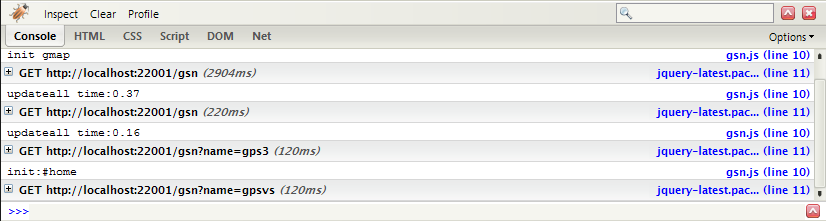
\includegraphics[width=1\textwidth]{firebug.png} \end{center}

As shown above, it allows easy debugging message using the \emph{console.debug(...)} object. Object can be fully analysed and changed. The html and css code could be modified on the fly. This is very powerful and helps a lot. 

Nevertheless, when testing gsn compatibility with IE, this is a pain to not have FireBug. Moreover that IE usually have some weird and hard to catch javascript bug.


\subsection*{GPSVS sensor}

During the project, we received a GPS bluetooth sensor. Being highly interested to test it with the brand new google map interface of gsn and to check the accuracy, I developed a quick virtual sensors and xml file for it. Using the serial port wrapper, it was very fast and easy and allowed me to get a better knowledge of the gsn middleware architecture. It also bring some relevant feedback to the team. The sensor code was quickly put together using a serial port wrapper, as bluetooth support serial port emulation. GPS sensor actually have some specification for their output called NMEA\cite{nmea}. Only a subset of it was implemented, the GPRMC part to be precise. This is some formatted text only output looking for example like \emph{"\$GPRMC,081836,A,3751.65,S,14507.36,E,000.0,360.0,130998,011.3,E*62"} which has to be converted to Google maps coordinate.

The GPS sensor was developed using a GPSlim device but should be successfully used by any device following the NMEA specification. It was actually tested with a Nokia GPS device without any modification. The only small problem was the linkage of the Nokia GPS device which require a passcode. It can be found deep down in the documentation and is 0000 by default.  

\subsection*{Ruby on Rails}

In the first week of January, I had a brief overview of Ruby on Rails. It is an interesting framework with lot of potential. However, I haven't had a chance to produce anything useful as one week later, I want back to finish some last requirement to the gsn webapp. 

\subsection*{Conclusion}

Overall, I have enjoyed this semester project. My knowledge of Javascript greatly improved and the jQuery library that I had never used reveled to be very powerful. There were some challenging problems and discussion. Moreover, I'm glad that this project seems to be starting out to gain an user base, which means the code I wrote will be useful to many. I'm happy with what I've achieved and hope the webapp will continue to be improved.

Communication with the assistant were fine as we had numerous meeting and emails. On the other hand, communication with the other students were very brief as we divided the work to have distinct part and avoid overlap.

I've particularly enjoyed doing the GPS sensor implementation which wasn't formerly part of my project but allowed me to gain inside knowledge of the gsn framework as a whole. It gave me a much better view of the system and it usefulness. I've only spent like one evening on it, but it was much fun.

I hope the gsn project will continue to grow and that the directory will be a success. Hopefully, the following students will improve it further. I will certainly keep an eye on it. 


\newpage
\begin{thebibliography}{77}
\bibitem{ajax} AJAX, \url{http://adaptivepath.com/publications/essays/archives/000385.php}
\bibitem{jquery} JQuery, {\it  New Wave Javascript,} \url{http://jquery.com/}
\bibitem{prototype} Prototype, \url{http://prototype.conio.net/}
\bibitem{mootools} mootools, \url{http://mootools.net/}
\bibitem{yui} Yahoo! UI Library, \url{http://developer.yahoo.com/yui/}
\bibitem{nmea} NMEA sentence information, \url{http://www.werple.net.au/~gnb/gps/nmea.html}
\bibitem{firebug} FireBug, \url{http://www.getfirebug.com/}
\end{thebibliography}

\newpage
\section*{Annexe}

Some screen of the current web interface
\begin{center} 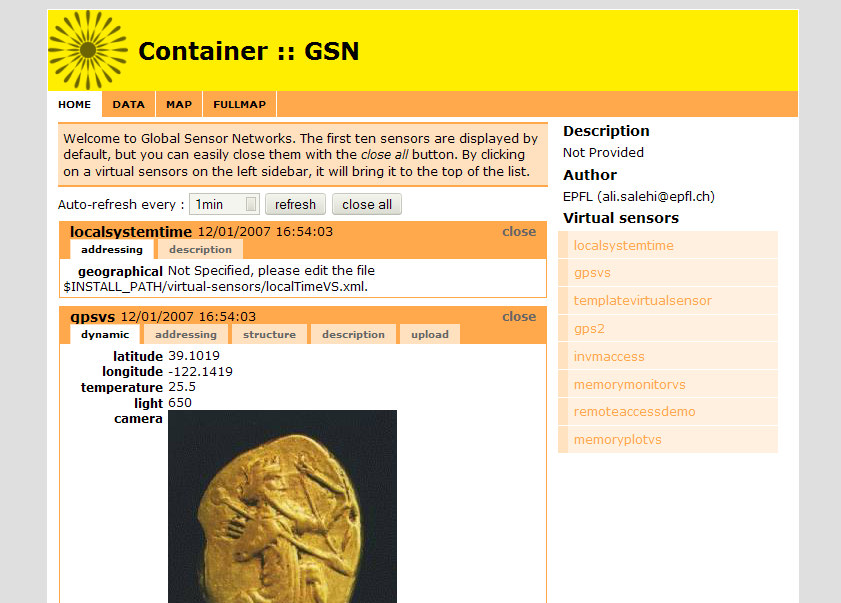
\includegraphics[width=0.8\textwidth]{gsn2_gsn.png} \end{center} 
\begin{center} 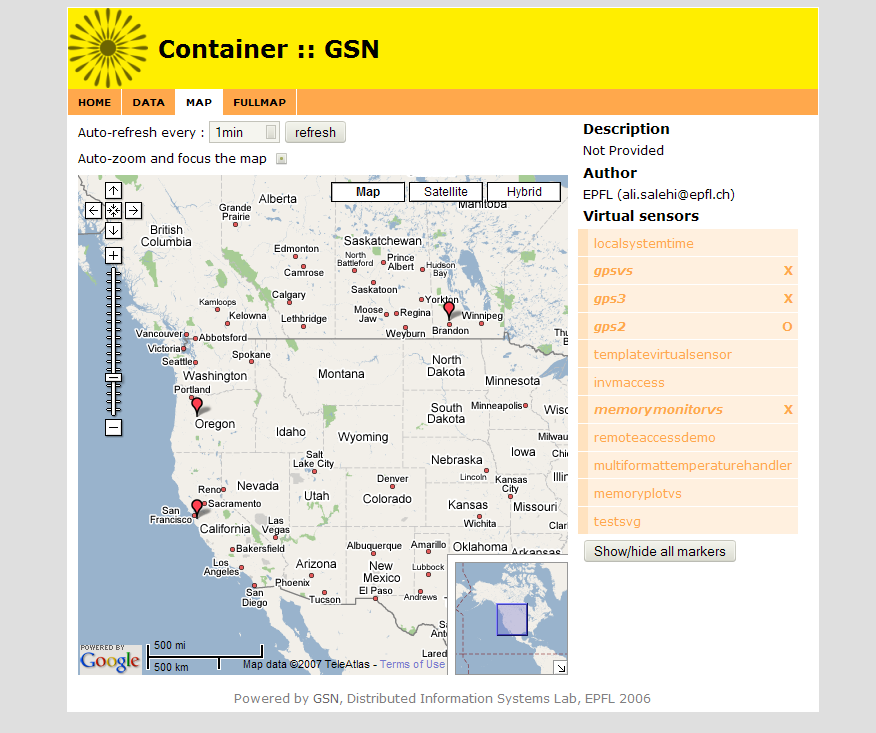
\includegraphics[width=0.8\textwidth]{gsn2_map.png} \end{center} 
\begin{center} 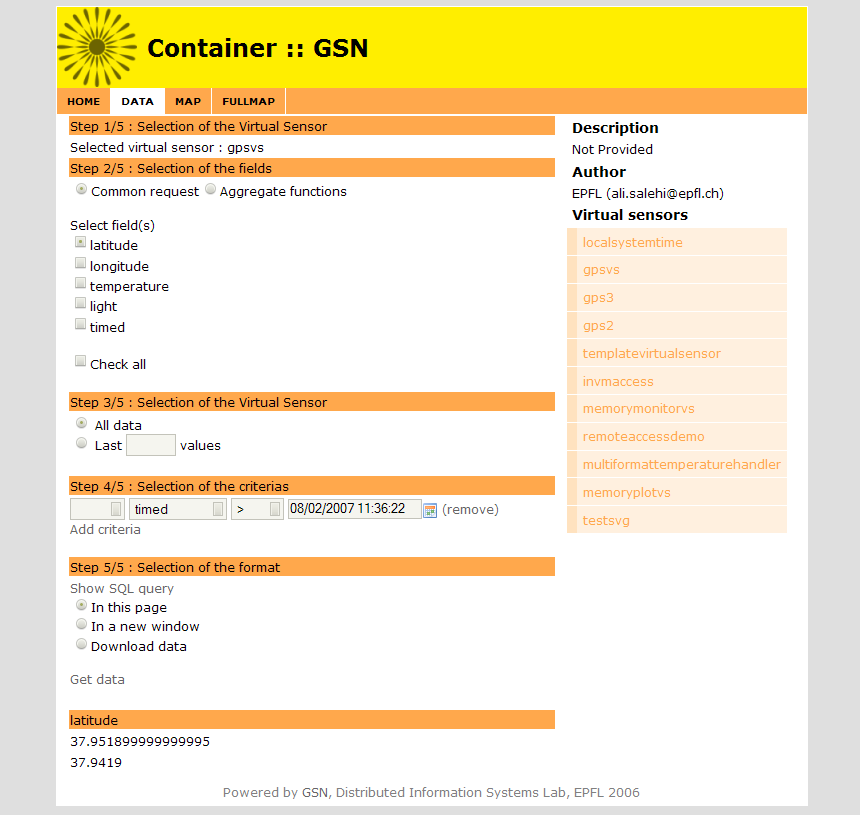
\includegraphics[width=0.7\textwidth]{gsn2_data.png} \end{center}
\begin{center} 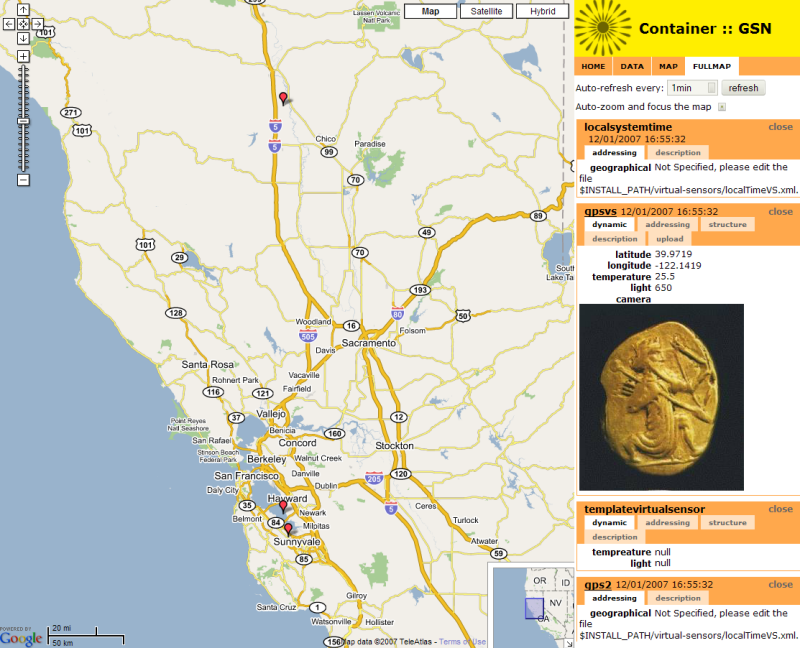
\includegraphics[width=0.8\textwidth]{gsn2_fullmap.png} \end{center}

\newpage
State of the web interface prior to the project
\begin{center} 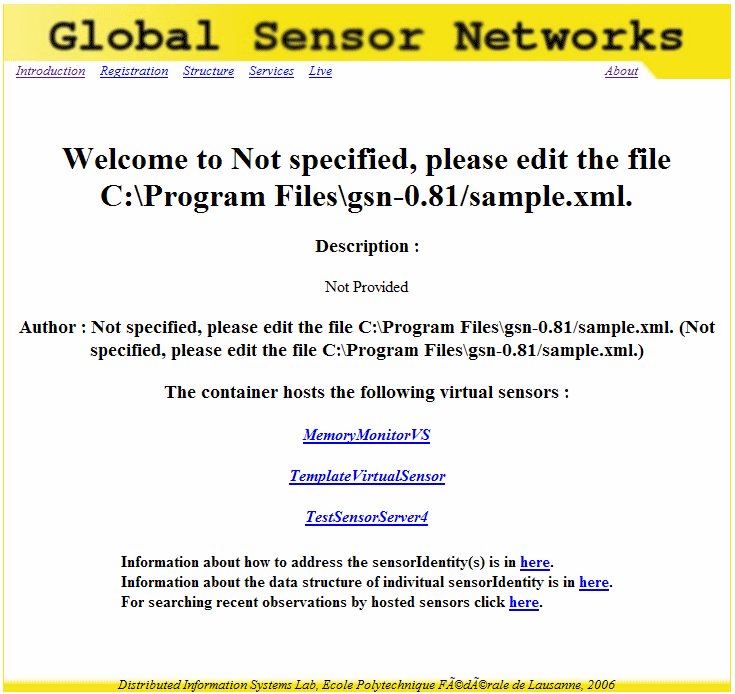
\includegraphics{gsn1_intro.png} \end{center} 
\begin{center} 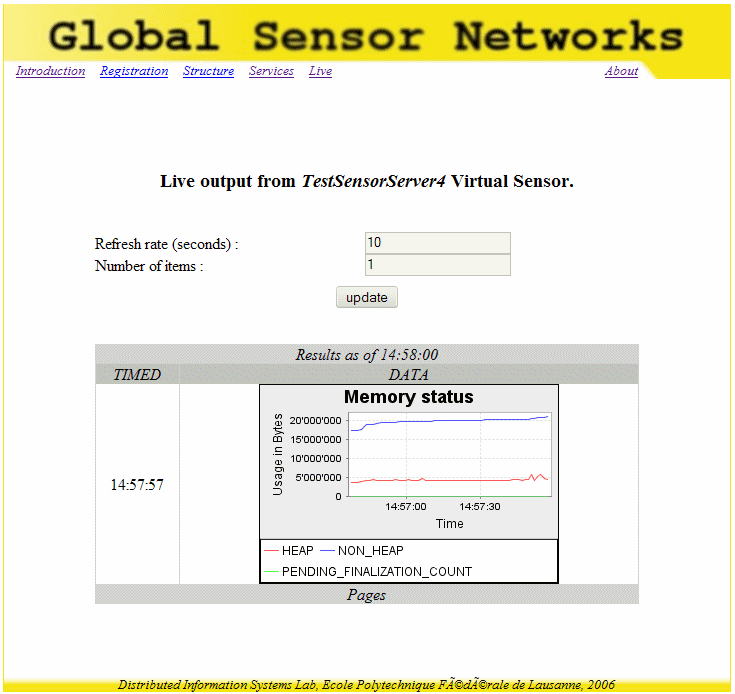
\includegraphics{gsn1_live.png} \end{center}

\newpage
Sample xml ouput from the web api servlet
\begin{verbatim}
<?xml version="1.0" encoding="ISO-8859-1"?>
<gsn name="Container" author="EPFL" email="ali.salehi@epfl.ch" 
description="Not Provided">
  <virtual-sensor name="gpsvs" last-modified="1171104402145" 
  description="Virtual sensor producing random locations">
    <field name="latitude" type="double" description="tested desc">37.45</field>
    <field name="longitude" type="double">-122.1419</field>
    <field name="temperature" type="double">25.5</field>
    <field name="timed" type="long" description="The timestamp associated 
    with the stream element">1171471973533</field>
    <field name="type" category="predicate">test-sensor</field>
	<field command="cmd1" name="test1" category="input" 
	type="radio:apple|orange|banana" description="one"></field>
	<field command="cmd1" name="test2" category="input" 
	type="*checkbox:apple|orange|banana" description="two"></field>
	<field command="cmd1" name="test3" category="input" 
	type="select:apple|orange|banana" description="three"></field>
  </virtual-sensor>
  <virtual-sensor name="gps25" last-modified="1171105163070" 
  description="Not Specified">
    <field name="timed" type="long" description="The timestamp associated
	with the stream element"></field>
    <field name="latitude" category="predicate">37.32</field>
    <field name="longitude" category="predicate">-122.1</field>
  </virtual-sensor>
</gsn>
\end{verbatim}

\newpage
Sample xml config of a virtual sensor with webinput capability:
\begin{verbatim}
<virtual-sensor name="gps1">
  <processing-class>
    <class-name>gsn.vsensor.BridgeVirtualSensor</class-name>
      <init-params/>
      <web-input password="test">
        <command name="cmd1">
          <field name="test1" type="radio:apple|orange|banana" >one</field>
          <field name="test2" type="*checkbox:apple|orange|banana" >two</field>
          <field name="test3" type="select:apple|orange|banana" >three</field>          
        </command>
        <command name="cmd2">
          <field name="reset1" type="byte" />
          <field name="reset2" type="*binary:2mb" >Files Size of 2MB</field>
        </command>
      </web-input>
      <output-structure>
         <field name="latitude" type="double" >test description</field>
      </output-structure>
  </processing-class>
  <description>Virtual sensor producing random locations</description>
  <addressing>
    <predicate key="longitude">149.1</predicate>
  </addressing>
  <storage history-size="1m"/>
  <streams>
    <stream name="input1">
      <source alias="source1" sampling-rate="1" storage-size="1">
        <address wrapper="system-time">
          <predicate key="HOST">localhost</predicate>
        </address>
        <query>select * from wrapper</query>
      </source>
      <query>select * from source1</query>
    </stream> 
  </streams>
</virtual-sensor> 
\end{verbatim}


\newpage
\subsection*{Using GSN web interface from another webserver}
GSN web interface can be integrated into another webserver running a CMS or wiki. It could be done using a IFrame or more closely by copying the html code and the JavaScript code. The webapp needs however access to the servlets. Ajax calls can not be done to a different host or port and therefore the servlet has to be mirrored in the webserver.

Under Apache, it can be done using a proxy. The following modules has to be enable in httpd.conf.

\begin{verbatim}
LoadModule proxy_module modules/mod_proxy.so
LoadModule proxy_http_module modules/mod_proxy_http.so
LoadModule rewrite_module modules/mod_rewrite.so
\end{verbatim}

The gsn servlets are mirrored using the following rewrite rule. It should be added in the DocumentRoot part of httpd.conf.

\begin{verbatim}
<Directory "...">
	RewriteEngine on
	RewriteRule ^(gsn|field|data|upload)(|\?(.*))$ http://localhost:22001/$0 [P]
</Directory>
\end{verbatim}

Finally, \emph{index.html} and \emph{fullmap.html} have to be edited to change the Google map API key for their new location.


\end{document}